%\graphicspath{{chapters/images/28032022/}}

If you want to maximize the output, you don't have to maximize the expression. Optimization strategies are
Logic gates with plasmids, sometimes works, some other times not. Only we care about logic gates, as biology doesn't work with them. 

Plasmids:
provide a dynamic and quick
response to environmental pressure, make the introduction of genetic circuitry
easy,
exact cost from the host cell, difficult to control, not sustainable,
movable genetic elements. 
Sust


Flux making inbolves different problems: not completely determined, consequently there will be a lot of uncertainty. 


Noisy systems, selectable metabollic elements, survive unfavourable environments by chance. 

Some kind of output fluorescence to monitor reactions. Reporter fluorescent proteins. 



Different types of standardizations are needed, to make biology more quantitative and engineer-similar.
can we standardize the strength of promoters, operators for regulation, RBS, plasmid copy number is also important to be standardized. \\
REU is a quantitative measure f the system (). Three different type of chambers, they wanted to standardize the output from the same genetic system, reference plasmid. 
The idea is to understand the complexity of biologyical system (black box), in order to understand the output of a specific input.
A and B not only have to be in same system, also output input required matched. 

Nature naturally works in a different way if compared to engineering:
– mutations,
– loss of plasmids,
– leaky expression,
– metabolic burden, slow growth, death
– requirement of higher amount or nutrients
(higher cost).
– network connectivity

\section{Directed Evolution}
for example, consume a toxic metabolite. You induce variation in the system through diversification. The system has to come up with a solution which permits to select a variant, that can be selected (better and better). white dots changes in different directions, 

\begin{figure}[h]
\caption{}
\centering
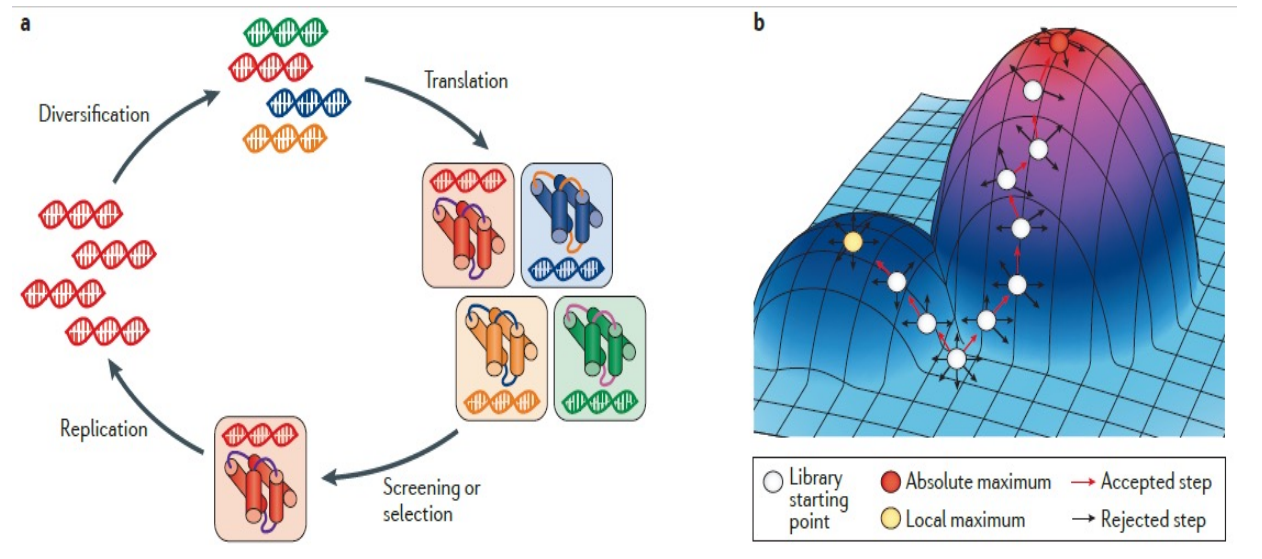
\includegraphics[width=0.6\textwidth]{directed evolution}
\label{}
\end{figure}

\begin{figure}[h]
\caption{epPCR the enzyme is ok, the conditions are fucked up}
\centering
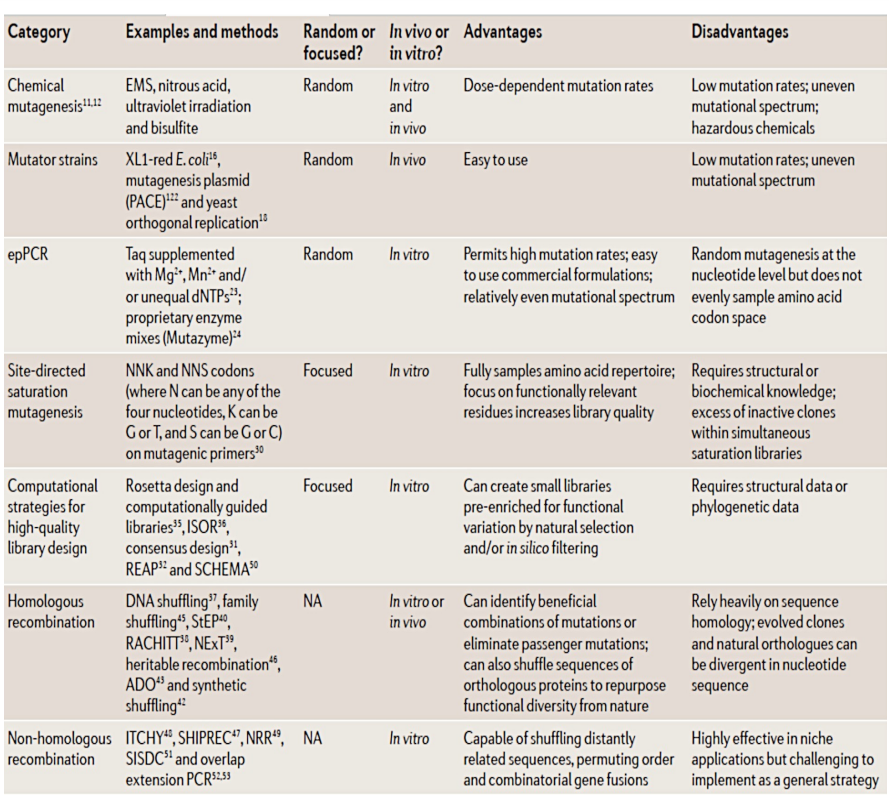
\includegraphics[width=0.6\textwidth]{mutagenesis_induced}
\label{}
\end{figure}

Each of the variants are tried. The mutation imposed could be random or focused, depending on the need. It can be done then \textit{in vivo} or \textit{in vitro}. random mutagenesis can be done by using physical tools, like radiation. 


Screening and selection can be done through bacteria coltures mass spectrometry and measure fluorescence

\begin{figure}[h]
\caption{}
\centering
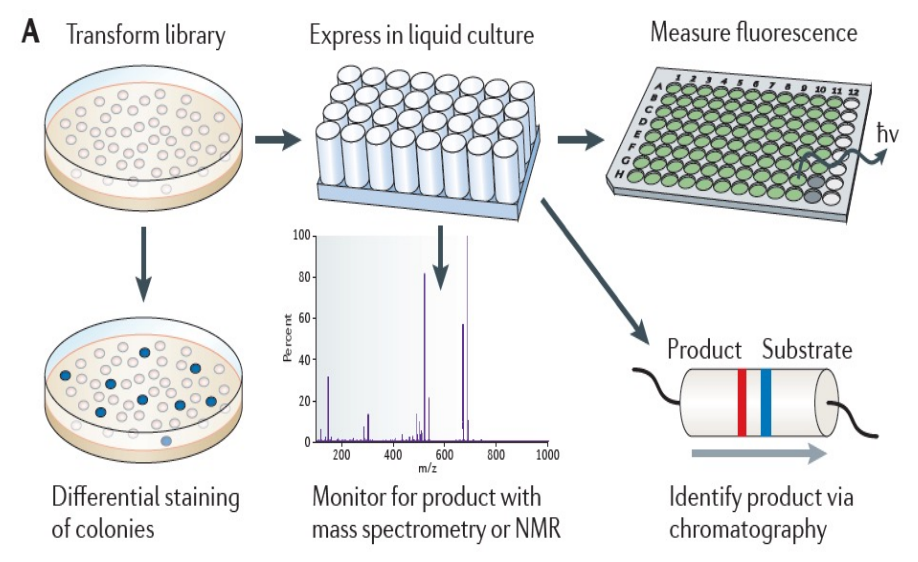
\includegraphics[width=0.6\textwidth]{screenSel}
\label{}
\end{figure}

with flow citometry, it's possible to select a precise cell population.\\
\\
The other way would be to modify the action of enzymes. mutate enzyme, screen it, take the one which produces the best output. Unfortunately, ti is not possible today to predict the structure of a protein by making simple changes. It has to be coupled the genotype with the phenotype. \\
How you link informations?

in the image, there's an immobilized target, protei binds to it and I don't know it. M13 phage engineerde to express a specific molecule. Select phages that are teally ood in binding the target. 

\begin{figure}[h]
\caption{selecting for things "sticky", ensure stickyness is enougly high}
\centering
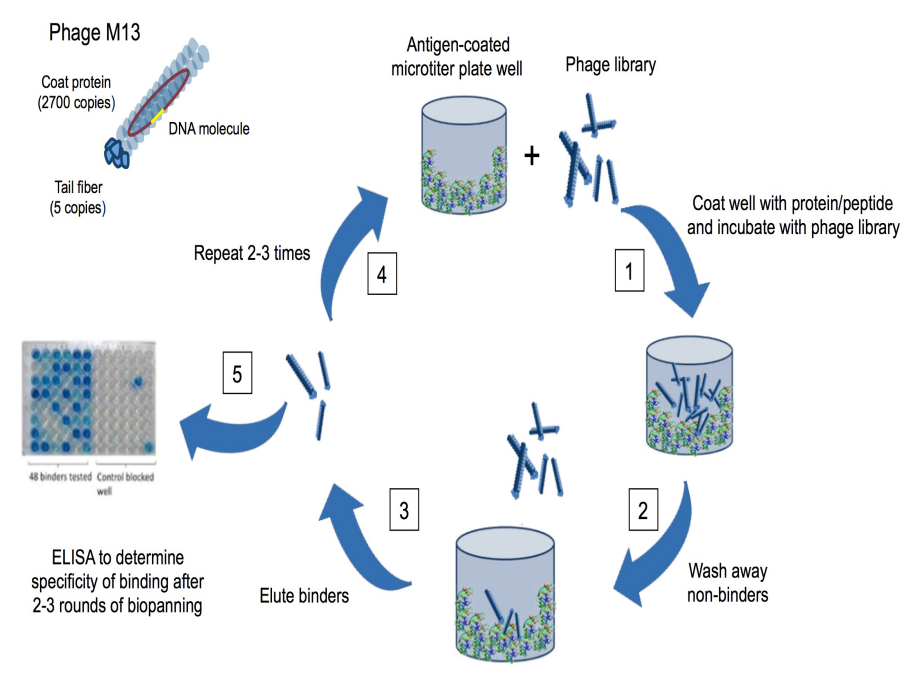
\includegraphics[width=0.6\textwidth]{phageM13}
\label{}
\end{figure}

Puromycin/mRNA. mRNA bound to puromycin.

Rybosom bound to mRNA functions really similarly.  

\section{Ribozymes}
the reaction of splicing consumes itself, it happens just one time. Using an external G, it is possible to have an IVS region.

\begin{figure}[h]
\caption{}
\centering
\includegraphics[width=0.6\textwidth]{exoG}
\label{}
\end{figure}


